
\section{Appendix}
\label{app:a}

\subsection{Other Approaches for Preferences in Argumentation Frameworks}
\label{app:other_afs}
\label{sub:paf}
Other approaches to deal with preferences in argumentation frameworks have been proposed by \cite{amgoud,amgoud1998,Bench2003,pollock1987, prakken1997}. A \gls{PAF} defined in \cite{amgoud1998} is  a triple $\langle \S, \R, Pref \rangle$ where $Pref$ is a (partial of complete) order preordering on $\S \times \S$. The difference between this approach and the one we use is mostly the requirement of a strict ordering that has to be associated with $Pref$ and must be explicitly defined.

Modgil \textit{et al.} introduce in \cite{Modgil2009} the concept of a special class of \textit{hiearchical \glspl{EAF}}, which are defined by the existence of a partition of $\Delta$ into multiple regular Dung argumentation frameworks. Due to this restriction it is possible to define a least fix point of the characteristic function $F$, hence defining the grounded extension $GE(\Delta)$ in the same way, as it has been defined in Dung's framework. However, this is a to narrow restriction for our purposes, therefore this will not be described here. 

\label{sub:vaf}

\Glspl{VAF} as proposed in \cite{Bench2003} define an argumentation framework as a 5-tuple: $\langle \S, \R, V, val, P \rangle$ ($\S$: Arguments, $\R$: Attack relation, $V$: nonempty set of values, $val(\cdot): \S \rightarrow V$: value mapping function, $P$: set of audiences $\{a_1, ..., a_n\}$ where each audience names a total ordering $>_{a_i}$ on $V \times V$). By referring to one specific audience we retrieve a \gls{aVAF}. The set of audiences $P$ is introduced to be able to make use of preferences between values in $V$, so we might have as many audiences as there are orderings on $V$. The new definition of an argument that defeats another argument takes into account the audience $a$ and the $val(\cdot)$ of both arguments to define successful attacks. This approach requires a value mapping function $val(\cdot)$ and doesn't argue with preferences in a natural way. 

However, \cite{Modgil2009} proves that an \gls{aVAF} can be transferred to an \textit{equivalent} \gls{EAF} by representing the \gls{aVAF} with three layers: The outer layer expressing the audience, the second layer expressing the pairwise orderings on values in $V$, and the inner layer based on the actual arguments and attacks in the \gls{aVAF}.

Defeasible reasoning and preferences and their impact on argumentation frameworks are formalised as logical formalism by \cite{pollock1987, prakken1997} in the underlying logical formalism which will be used to instantiate a regular Dung framework.

\subsection{Sample Clinical Data Set}
\label{app:dataset}
{
	\centering
	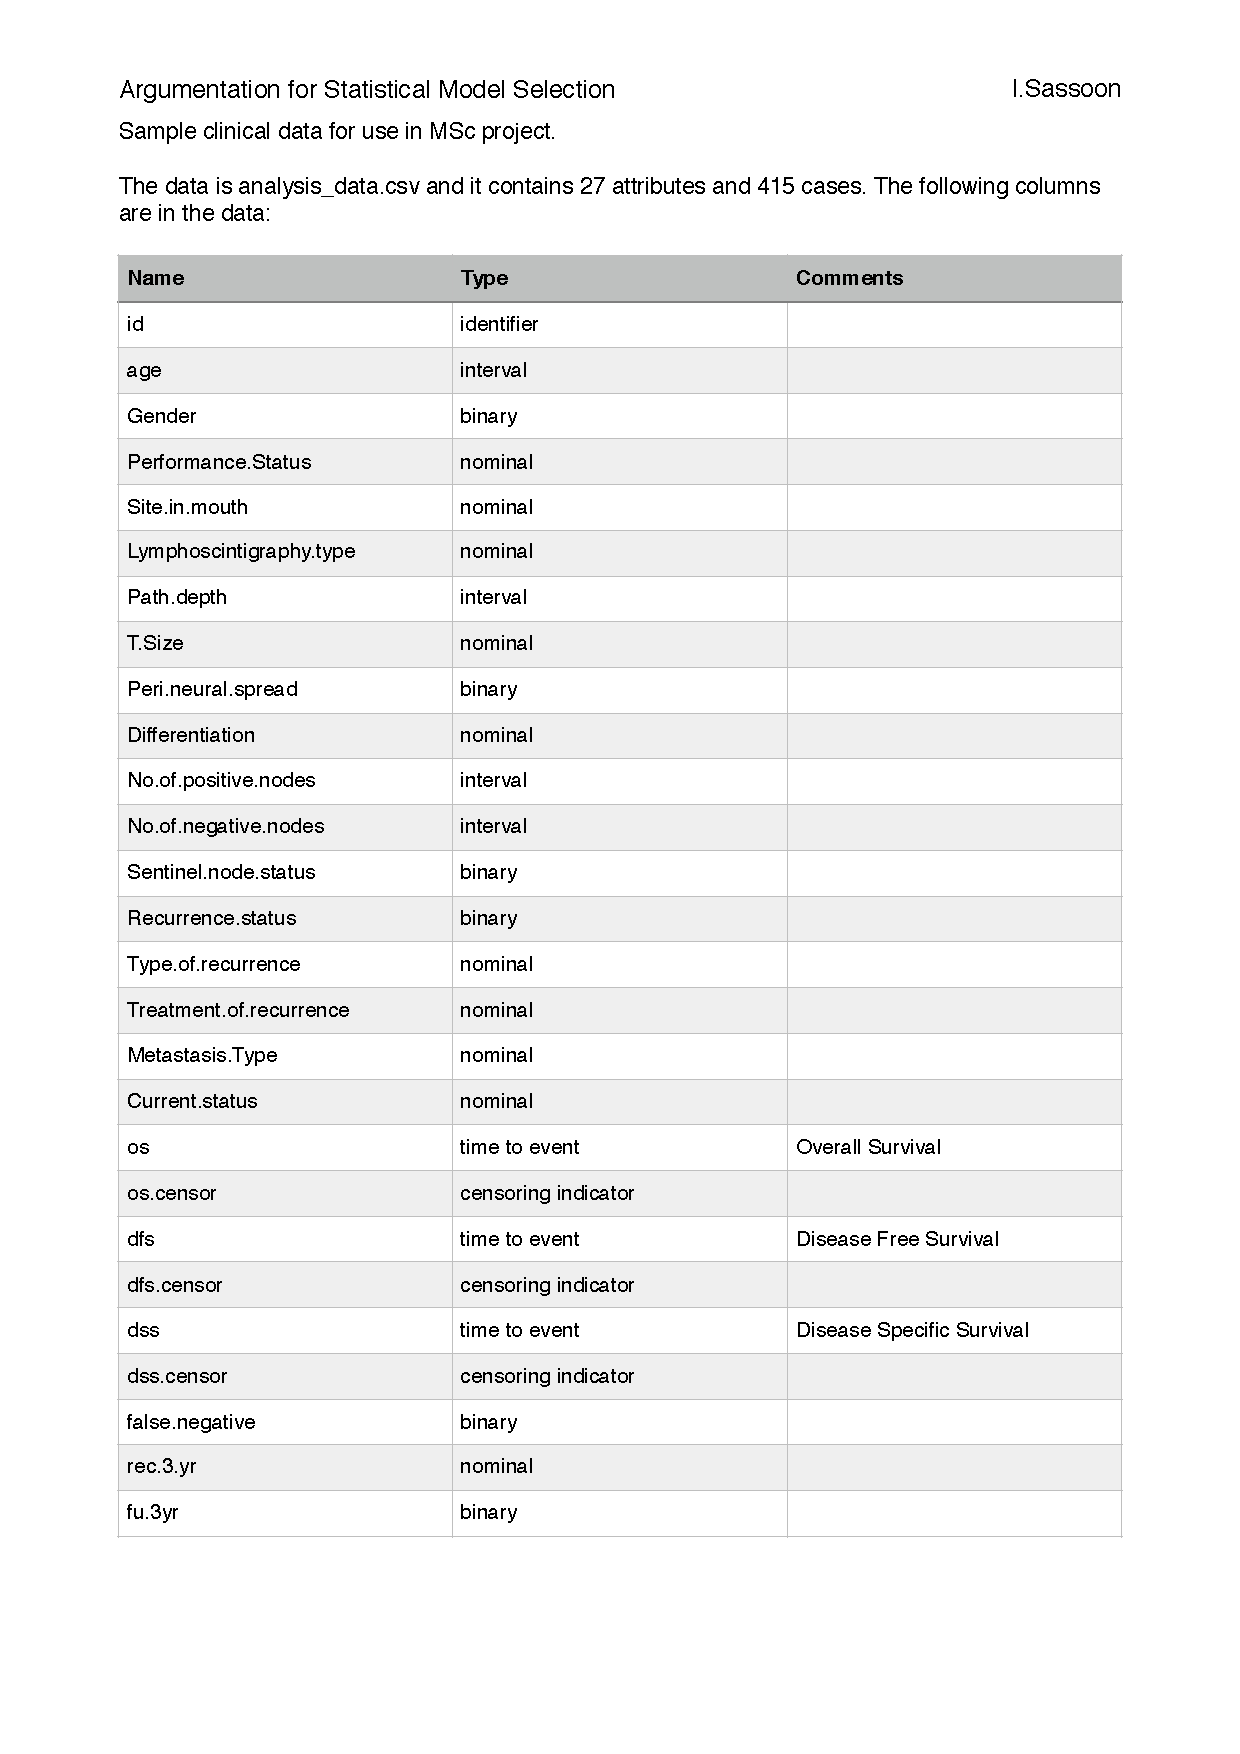
\includegraphics[page=1,width=0.85\textwidth]{appendix/analysis_data.pdf}
	\captionof{figure}{
	Explanation of the example data set provided by I. Sassoon (private email conversation)
	\label{fig:dataset}
	}

	\includegraphics[page=2,width=0.85\textwidth]{appendix/analysis_data.pdf}
	\captionof{figure}{Possible research questions arising from the example data set provided by I. Sassoon (private email conversation)
		\label{fig:dataset:rq}
	}
}



\section{Software related Appendix}
\label{app:b}
\subsection{Code Samples}

\begin{listing}[H]
	\centering
	\rubycode{figures/eaf_to_af.rb}	
	\caption{Ruby Code to implement \autoref{fig:eaf_algo}.}
	\label{lst:eaf}
\end{listing}

\begin{listing}[H]
	\centering
	\rubycode{figures/find_pref.rb}	
	\caption{Ruby Code to implement the labelling based approach $FIND\_PREF$ presented in \autoref{fig:af_algo}.}
	\label{lst:af}
\end{listing}

\begin{listing}[hbtp]
	\rcode{figures/weibull_test.r}
	\caption{R-script to perform a \texttt{QueryTestAssumption} on a data set to check whether the Weibull-Model is applicable or not. The script generates a plot that will be stored in \texttt{fileName} and presented to the end-user.}
	\label{lst:rcode}
\end{listing}


\subsection{Installation Guide}
\label{app:installation}
The following installation guide has been tested on a clean debian OS:

\begin{enumerate}
\def\labelenumi{\arabic{enumi}.}
\item
  Install \texttt{postgresql} and \texttt{R} with:
  \texttt{sudo\ apt-get\ install\ postgresql\ r-base}
\item
  Install \texttt{rvm} following \href{https://rvm.io/rvm/install}{this
  guide}.
\item
  Clone the repository:\\
  \texttt{git\ clone\ }\url{https://github.com/sebastianzillessen/small-data-analyst.git}
\item
  \texttt{cd\ small-data-analyst}
\item
  Install the required ruby version as prompted by rvm:
  \texttt{rvm\ install\ ruby-2.2.4}
\item
  Install bundler: \texttt{gem\ install\ bundler\ foreman}
\item
  Install all required gems: \texttt{bundle\ install}
\item
  Set the AWS credentials in the file \texttt{.env}:

\begin{verbatim}
PORT=3000
AWS_ACCESS_KEY_ID=XXXXXXXXXXXXX
AWS_SECRET_ACCESS_KEY=YYYYYYYYYYYYYYYYYYYY
S3_BUCKET_NAME=ZZZZZZZZZZZZZZ
\end{verbatim}
\item Set the database credentials if required in \texttt{config/database.yml}.
\item
  Initialise the database:\\
  \texttt{rake\ db:create\ \&\&\ rake\ db:setup\ \&\&\ rake\ db:migrate}
\item
  Start the server with \texttt{foreman\ start}
\item
  Create an Admin user:

\begin{verbatim}
$ rails console
> u = User.create(email: "test1@test.de", password: "fooPassword", 
		approved: true, role: :admin)
> u.confirm!
\end{verbatim}
\item
  Navigate to \texttt{http://localhost:3000} and play around with the
  application.
\end{enumerate}


\subsection{Use Cases}
\label{app:use_cases}

Figures \ref{fig:usecase:clinician}, \ref{fig:usecase:statistician} and \ref{fig:usecase:admin} provide an overview over the implemented \glspl{use_case} in the application grouped by their main actors. A complete list of all use cases can be found for further references under \href{https://trello.com/b/ywCkicpc/msc-small-data-analyst}{https://trello.com/b/ywCkicpc/msc-small-data-analyst}.

% use_cases
{
	\centering
	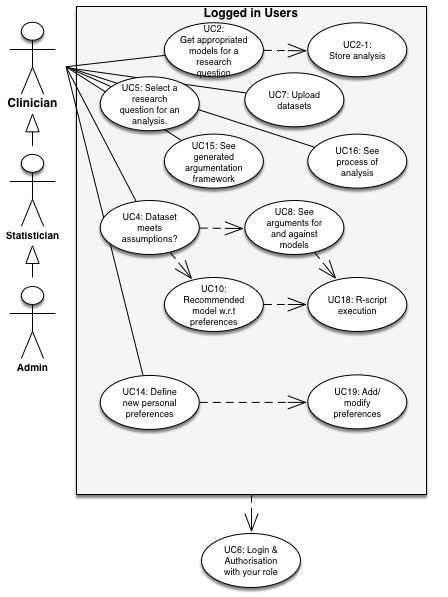
\includegraphics[width=0.6\textwidth]{figures/use_case_clinician}
	\captionof{figure}{Use Case overview for clinicians \label{fig:usecase:clinician}}
	
	
	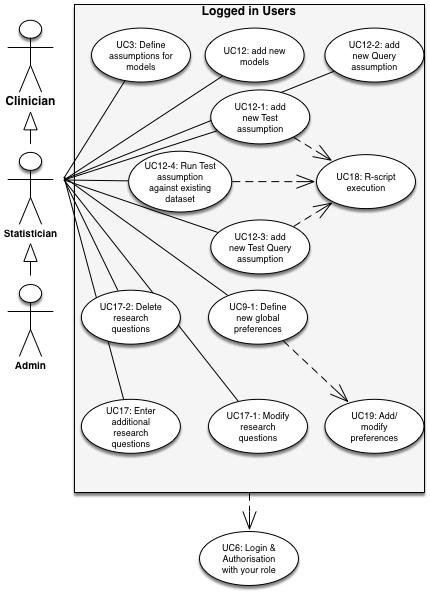
\includegraphics[width=0.6\textwidth]{figures/use_case_statistician}
	\captionof{figure}{Use Case overview for statisticians \label{fig:usecase:statistician}}
	
	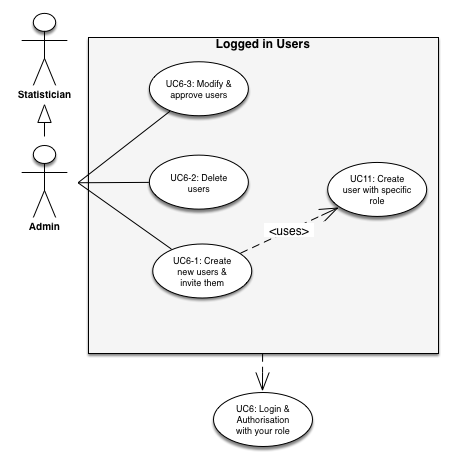
\includegraphics[width=0.6\textwidth]{figures/use_case_admin}
	\captionof{figure}{Use Case overview for administrators \label{fig:usecase:admin}}

}

\section{Third Party Libaries}
\label{app:c}
\label{app:3rdparty}
\autoref{tab:libs} contains all the third party libraries that have been used in the project. These are all public available and free of use. Additional information can be found for each listed \texttt{gem} under \href{http://rubygems.org}{http://rubygems.org}.

\begin{table}[!h]
	\centering
	\begin{tabular}{|p{2.4cm}r||p{2.4cm}r||p{2.4cm}r|}
	\hline
	\textbf{Library} & \textbf{ver.} & 	\textbf{Library} & \textbf{ver.} & 	\textbf{Library} & \textbf{ver.} \\
	actionmailer&(4.2.6)&faker&(1.6.3)&rails\_12factor&(0.0.3)\\
actionpack&(4.2.6)&foreman&(0.82.0)&\tiny{rails\_serve\_static\_assets}&(0.0.5)\\
actionview&(4.2.6)&formtastic&(3.1.4)&\tiny{rails\_stdout\_logging}&(0.0.5)\\
activejob&(4.2.6)&\tiny{formtastic-bootstrap}&(3.1.1)&railties&(4.2.6)\\
activemodel&(4.2.6)&globalid&(0.3.6)&rake&(11.2.2)\\
activerecord&(4.2.6)&haml&(4.0.7)&rdoc&(4.2.2)\\
activesupport&(4.2.6)&haml-rails&(0.9.0)&ref&(2.0.0)\\
addressable&(2.4.0)&heroku-api&(0.4.2)&responders&(2.2.0)\\
arel&(6.0.3)&html2haml&(2.0.0)&\tiny{rootapp-rinruby}&(3.1.2)\footnote{https://github.com/sebastianzillessen/rinruby}\\
aws-sdk&(2.4.2)&i18n&(0.7.0)&rspec-core&(3.4.4)\\
aws-sdk-core&(2.4.2)&jbuilder&(2.5.0)&\tiny{rspec-expectations}&(3.4.0)\\
\tiny{aws-sdk-resources}&(2.4.2)&jmespath&(1.3.1)&rspec-mocks&(3.4.1)\\
bcrypt&(3.1.11)&jquery-rails&(4.1.1)&rspec-rails&(3.4.2)\\
\tiny{binding\_of\_caller}&(0.7.2)&\tiny{jquery-turbolinks}&(2.1.0)&rspec-retry&(0.4.5)\\
builder&(3.2.2)&jquery-ui-rails&(5.0.5)&rspec-support&(3.4.1)\\
bullet&(5.1.1)&json&(1.8.3)&ruby-graphviz&(1.2.2)\\
bundler&(1.12.5)&launchy&(2.4.3)&ruby\_parser&(3.8.2)\\
byebug&(9.0.5)&less&(2.6.0)&rush&(0.6.8)\\
cancancan&(1.15.0)&less-rails&(2.7.1)&sass&(3.4.22)\\
capybara&(2.7.1)&libv8&(3.16.*)&sass-rails&(5.0.4)\\
\tiny{capybara-screenshot}&(1.0.13)&loofah&(2.0.3)&sdoc&(0.4.1)\\
choice&(0.2.0)&mail&(2.6.4)&session&(3.2.0)\\
cliver&(0.3.2)&method\_source&(0.8.2)&sexp\_processor&(4.7.0)\\
cocoon&(1.2.9)&\tiny{mime-types}&(3.1)&\tiny{shoulda-matchers}&(3.1.1)\\
\tiny{codeclimate-test-reporter}&(0.6.0)&\tiny{mime-types-data}&(3.2016*)&simplecov&(0.12.0)\\
coderay&(1.1.1)&mini\_portile2&(2.1.0)&\tiny{simplecov-html}&(0.10.0)\\
coffee-rails&(4.1.1)&minitest&(5.9.0)&slop&(3.6.0)\\
coffee-script&(2.4.1)&multi\_json&(1.12.1)&sprockets&(3.6.2)\\
\tiny{coffee-script-source}&(1.10.0)&nokogiri&(1.6.8)&sprockets-rails&(3.0.4)\\
commonjs&(0.2.7)&orm\_adapter&(0.5.0)&teaspoon&(1.1.5)\\
\tiny{concurrent-ruby}&(1.0.2)&pg&(0.18.4)&\tiny{teaspoon-jasmine}&(2.3.4)\\
data\_migrate&(2.1.0)&pkg-config&(1.1.7)&therubyracer&(0.12.2)\\
\tiny{database\_cleaner}&(1.5.3)&poltergeist&(1.10.0)&thor&(0.19.1)\\
debug\_inspector&(0.0.2)&pry&(0.10.3)&thread\_safe&(0.3.5)\\
delayed\_job&(4.1.2)&puma&(3.4.0)&tilt&(2.0.5)\\
\tiny{delayed\_job\_active\_record}&(4.1.1)&rack&(1.6.4)&turbolinks&(2.5.3)\\
devise&(4.1.1)&\tiny{rack-mini-profiler}&(0.10.1)&\tiny{twitter-bootstrap-rails}&(3.2.2)\\
diff-lcs&(1.2.5)&rack-test&(0.6.3)&tzinfo&(1.2.2)\\plec
docile&(1.1.5)&rails&(4.2.6)&uglifier&(3.0.0)\\
dotenv&(2.1.1)&\tiny{rails-assets-chosen}&(1.6.1)&uniform\_notifier&(1.10.0)\\
dotenv-rails&(2.1.1)&\tiny{rails-assets-jquery}&(3.0.0)&warden&(1.2.6)\\
erubis&(2.7.0)&\tiny{rails-deprecated\_sanitizer}&(1.0.3)&web-console&(2.3.0)\\
excon&(0.51.0)&\tiny{rails-dom-testing}&(1.0.7)&\tiny{websocket-driver}&(0.6.4)\\
execjs&(2.7.0)&rails-erd&(1.4.7)&\tiny{websocket-extensions}&(0.1.2)\\
factory\_girl&(4.7.0)&\tiny{rails-html-sanitizer}&(1.0.3)&workless&(1.2.3)\\
factory\_girl\_rails&(4.7.0)&&&&\\
	\hline
	\end{tabular}
	\caption{Third-party libraries and services used in the web-application.}
	\label{tab:libs}
\end{table}

\clearpage
\newpage

\section{R-Spec Test Suite}
\label{app:d}
\label{app:rspec}
\sloppy
\autoref{sub:test_suit} provides an impression on the developed \texttt{rspec} tests. Only the first two pages have been generated. The whole report can be found on \href{https://github.com/sebastianzillessen/small-data-analyst/blob/master/report.html}{https://github.com/sebastianzillessen/small-data-analyst/blob/master/report.html}. The test suite which is made out of $\approx 350$ specs results in a resonable test coverage of $\geq 85\%$ (see \href{https://codeclimate.com/github/sebastianzillessen/small-data-analyst/coverage}{https://codeclimate.com/github/sebastianzillessen/small-data-analyst/coverage} for in depth code climate details and coverage report).
% rspec
\begin{sidewaysfigure}[!h]
	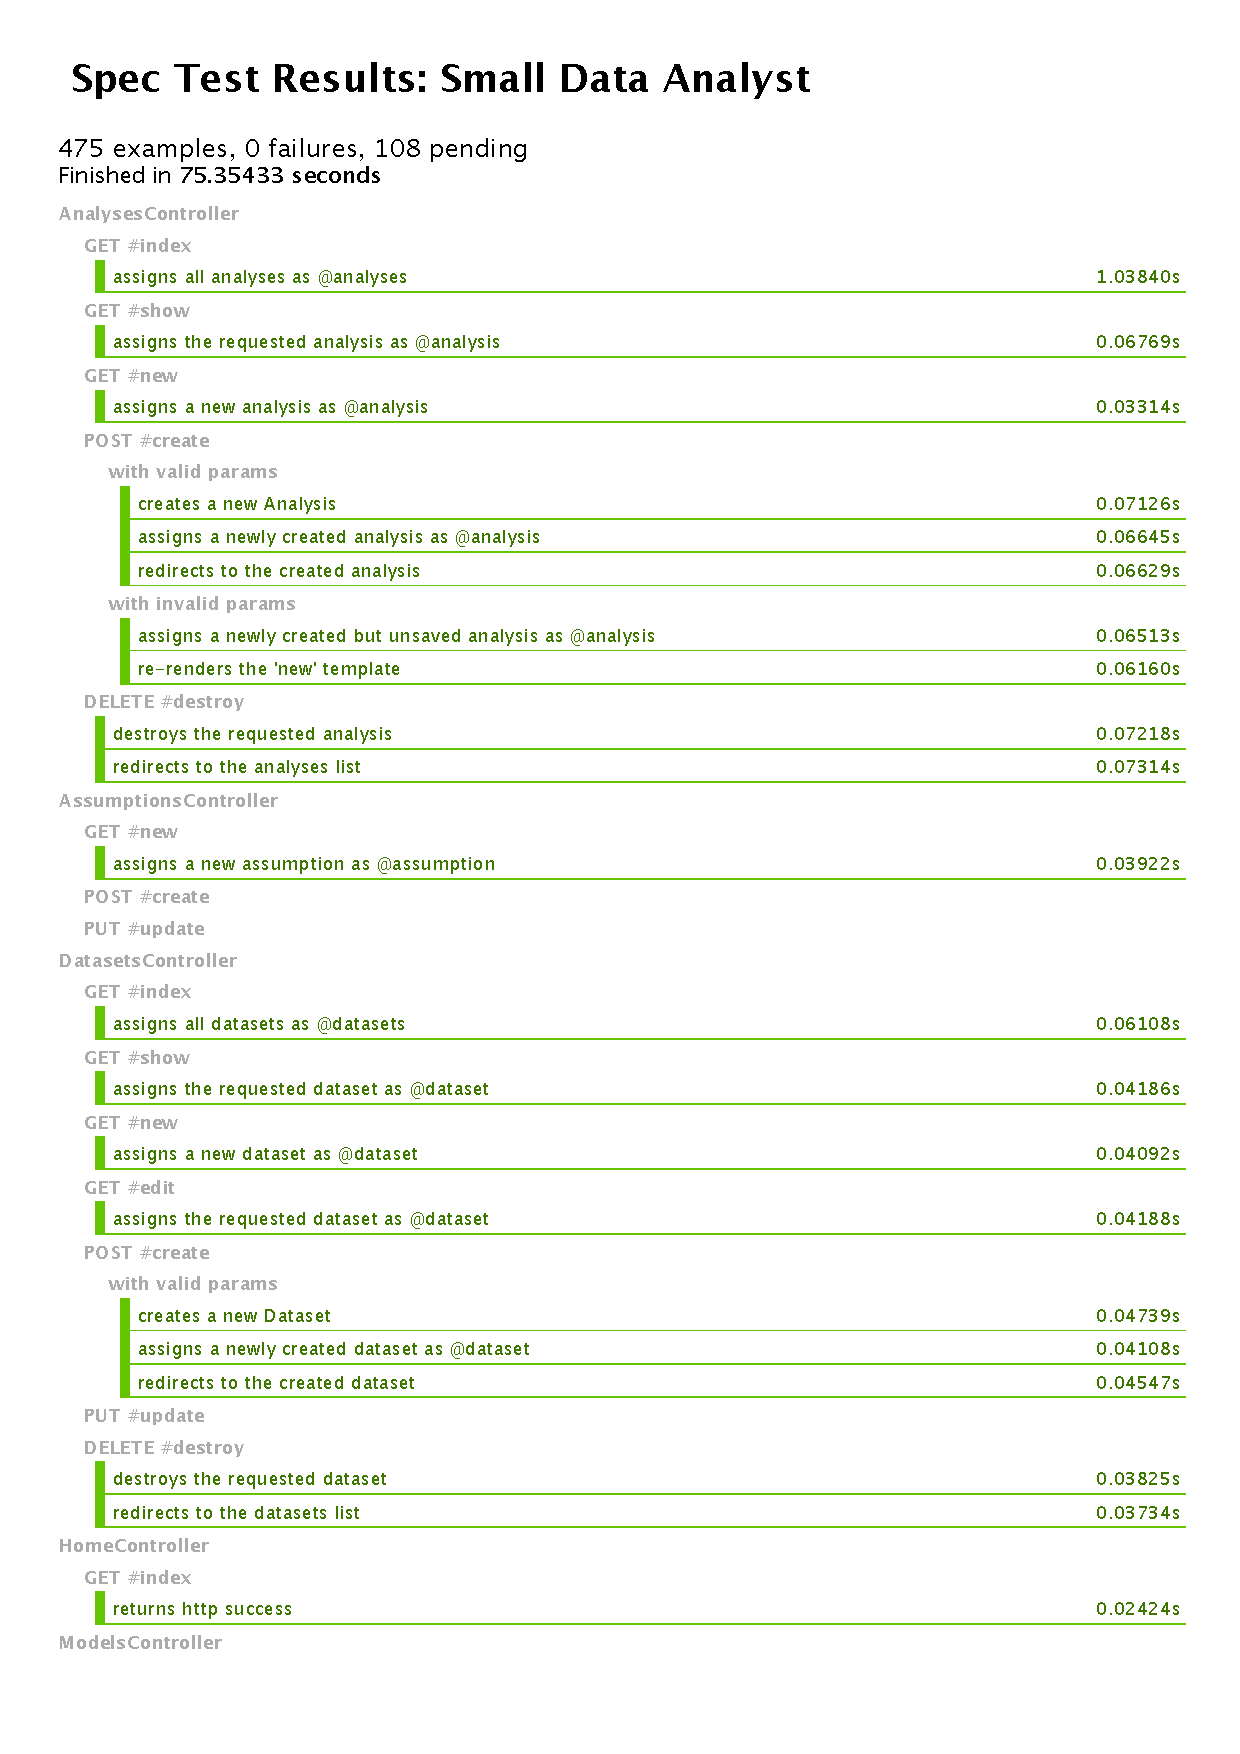
\includegraphics[page=1,width=0.5\textwidth]{appendix/RSpec}
	\includegraphics[page=2,width=0.5\textwidth]{appendix/RSpec}
	\caption{RSpec test suite export (example of the first two pages).}
	\label{sub:test_suit}
\end{sidewaysfigure}




